\documentclass[12pt]{report}
\usepackage{graphicx}
\usepackage{scribe_MG}
\usepackage{amssymb}
\usepackage{graphicx}
\usepackage[mathscr]{eucal}
\usepackage[english]{babel}
\usepackage[utf8]{inputenc}  %encodage du fichier
\usepackage[T1]{fontenc}
\usepackage{lmodern}
\usepackage{epstopdf}
\usepackage{array}
\usepackage{mathabx}

\usepackage{placeins}
\usepackage{enumerate}
\usepackage{commath}
\usepackage{amssymb}

%% William
\usepackage[colorlinks]{hyperref} % for links
\usepackage{xcolor}             % for color
\usepackage{caption}            % for caption* (without 'Figure 2.n:')
\usepackage{float}              % for H, to place figure HERE!
\usepackage{wrapfig}
\usepackage{tikz}
\usetikzlibrary{arrows}
\usetikzlibrary{positioning}

\usepackage{bbm}            % for the indicator function symbol : \mathbbm{1}
\def\R{\mathbb{R}}
\newcommand{\defobj}[1]{\color{red}#1\color{black}{}}
\newcommand{\defmean}[1]{\color{green!70!black}#1\color{black}{}}
\renewcommand{\emph}[1]{\color{violet}#1\color{black}{}}
\DeclareMathOperator{\E}{\mathbb{E}}

\newcommand{\sigmaField}{\mathcal{E}}

%% For footnote horizontal spacing :
%% \usepackage{footmisc}
%% \setlength{\footnotemargin}{2mm}

\newcommand\independent{\protect\mathpalette{\protect\independenT}{\perp}}
\def\independenT#1#2{\mathrel{\rlap{$#1#2$}\mkern2mu{#1#2}}} 

\newcommand{\indep}{\ensuremath{\,\bot\!\!\!\bot\,}} %% The symbol for independent
\newcommand{\notindep}{\indep\!\!\!\!\!/\,\,\,}

\newtheorem{remark}{Remark}[section]
\newtheorem{example}{Example}[section]
\newtheorem{property}{Property}[section]


\begin{document}
\coursetitle{IFT 6269: Probabilistic Graphical Models}
\semester{Fall 2016}
\lecturer{Simon Lacoste-Julien} \scribe{Sébastien Lachapelle}
\lecturenumber{5} \lecturedate{September 19}

\maketitle

\textbf{Disclaimer:} These notes have only been lightly proofread.

\section{Statistical Decision Theory}

\subsection{The Formal Setup}
Statistical decision theory is a formal setup to {\it{analyze}} decision rules in the context of uncertainty. The standard problem in statistics of estimation and hypothesis testing fit in it, but we will see that we can also the supervised learning problem from machine learning in it (though people are less used to see this in machine learning).

Let $D$ be a random observation (in ML, it would be a {\it training dataset}, which is why we used $D$). Let $\mathcal{D}$ be the sample space for $D$ (the set of all possible values for $D$). $D \in \mathcal{D}$. We say that $D \thicksim P$ where $P$ is a distribution over the set $\mathcal{D}$. We suppose that $P$ belongs to a certain set of distribution $\mathcal{P}$. We sometimes have that the distribution is parametrized by a parameter $\theta$ in which case we note this distribution $P_{\theta}$. $P$ represents the (unknown) state of the world (there is the source of uncertainty). \\

\noindent Let $\mathcal{A}$ be the set of all possible actions. We will denote $a$ a certain action in $\mathcal{A}$.\\

\noindent Let $L:\mathcal{P} \bigtimes \mathcal{A} \mapsto \mathbb{R}$ be the (statistical) loss function. So $L(P,a)$ is the loss of doing action $a$ when the actual distribution is $P$ (when the world is $P$).\\

\noindent Let $\delta:\mathcal{D} \mapsto \mathcal{A}$ be a decision rule.\\

Less formally, we observe something ($D$) from nature ($P$), but we do not actually know how mother nature generates observations (We don't know $P$). Even so, we suppose that $P$ belongs to a certain set of distribution ($\mathcal{P}$). We are in a context where we have to choose an action ($a$) among a certain set of actions ($\mathcal{A}$). Given the facts that we choose action $a$ and that the actual reality is $P$, we must pay a certain cost $L(P,a)$. Since we get to observe  a realisation of $P$, it makes sense to base our action on this observation. This decision process is described by $\delta$.\\

Important subtle point: often $P$ will describe an i.i.d. process, e.g. $D = (X_1,...,X_n)$ where $X_i \thicksim^{iid} P_0$. In this case, we often just write the dependence of the loss in terms of $P_0$ instead of the full joint $P$, i.e. $L(P,a) = L(P_0,a)$. Note that the framework also works for non i.i.d. data, but in this lecture we only consider i.i.d. data, and so when we write $L(P,a)$, we mean $P$ as a distribution on $X_i$, not the joint one...

\subsubsection{Examples}
\begin{enumerate}[A)]
\item \emph{Estimation}:\\
Suppose $P_{\theta}$ belongs to a parametrized family of distribution we call $\mathcal{P}$. We say that $\theta$ belongs to a parameter space denoted by $\Theta$. We pose $\mathcal{A}=\Theta$. In this context, $\delta$ is an estimator of $\theta$. We pose the following loss function (the famous "squared loss"):
$$L(P_{\theta}, a) = \norm{\theta - a}^2_2$$
We sometimes note $L(\theta, a)$ instead of $L(P_{\theta}, a)$ where this simplification applies. Remember that $\delta(D) = a$. In this specific case, we can write $\delta(D) = \hat{\theta}$.\\
We can suppose more specifically that $D = (X_1,...,X_n)$ where $X_i \thicksim^{iid} P_\theta$. This mean we would have:
$$L(\theta, \delta(D))=\norm{\theta - \delta(D)}^2_2$$
As a concrete example, suppose that $P_\theta$ belongs to a Gaussian family $\mathcal{P}=\{\mathcal{N}(\bullet\ ;\mu,1)|\ \mu \in \mathbb{R}\}$.
It would mean that $\Theta=\mathbb{R}$. For example, we could choose our decision function to be $\delta(D)=\frac{1}{n}\sum_i X_i$.
\item \emph{Hypothesis Testing}:
$\mathcal{A}=\{0,1\}$ where $0$ might mean not rejecting the null hypothesis and $1$ might mean accepting it. In this context, $\delta$ describes a statistical test.
\item \emph{Machine Learning for prediction}:\\
Let $D=((X_1,Y_1),...,(X_n,Y_n))$. We have that $X_i \in \mathcal{X}$ and that $Y_i \in \mathcal{Y}$ for all $i$. We call $\mathcal{X}$ the input space and $\mathcal{Y}$ the output space. Let $(X_i,Y_i) \thicksim^{iid} P_0$. Then $D \thicksim P$ where $P$ is the joint over all the i.i.d. $(X_i,Y_i)$ couples. $\mathcal{A}=\mathcal{Y}^\mathcal{X}$ (the set of functions who maps $\mathcal{X}$ to $\mathcal{Y}$). \\
In the prediction setting, we define a \textit{prediction loss function} $l:\mathcal{Y}^2 \mapsto \mathbb{R}$. This function is usually a measure of the distance between a given prediction and it's associated ground truth.\\
The actual loss function we would like to minimize is
$$L(P,f)=\E_{P_0}[l(Y,f(X))]$$
This is traditionally called the \textit{generalization error}, and is also often called the \textit{risk} in machine learning. Simon calls it the \textit{Vapnik risk} to distinguish it from the (frequentist) \textit{risk} from statistics that we will define later.

In this context, the decision rule $\delta$ is actually a learning algorithm that outputs a function $\hat{f} \in \mathcal{Y}^\mathcal{X}$. Equivalently, we can write that $\delta(D)=\hat{f}$.
\end{enumerate}

\subsection{Procedure Analysis}

Given this framework, how can we compare different rules (ie. procedures)? Given $\delta_1$ and $\delta_2$, how can I know which is better for a given application?
\subsubsection{(Frequentist) Risk}
The first property to analyze a procedure is called the \textit{risk} (or the \textit{frequentist risk}):
$$R(P,\delta) \triangleq \E_{D \thicksim P}[L(P,\delta(D)]$$

Remarks: The \textit{risk} is a function of $P$ and we don't know what $P$ is (in practice). So we never really know what's the value of this function for a given rule $\delta$. On the other hand, this property is a \textit{theoretical analysis device}: we can make statement like for $P$ in some family $\mathcal{P}$, procedure $\delta_1$ has lower risk than procedure $\delta_2$ (and is thus better in some sense). Also it is important to distinguish the (frequentist) \textit{risk} from the \textit{generalization error} (the Vapnik risk). \\

In the next graph, we expose the \textit{risk profiles} of two rules. For simplicity, we suppose that $P_\theta$ is a parametrized distribution and that $\theta \in \mathbb{R}$.

\centerline{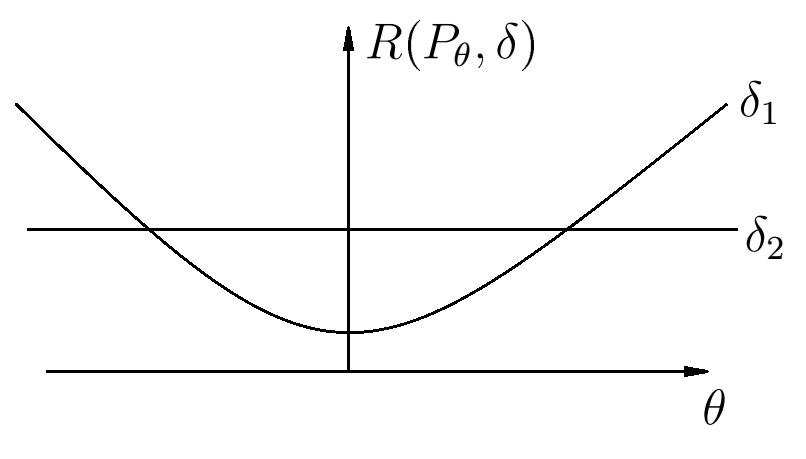
\includegraphics[scale=0.3]{graph_1.png}}

This picture illustrates the fact that sometimes, there is no clear winner when comparing two rules. In this case, it seems that $\delta_1$ is the best choice for values of $\theta$ near $0$. But for values of $\theta$ far from $0$, $\delta_2$ is the best choice. The problem is, we don't know the value of $\theta$, so we don't know the best rule to pick. We will see later that there are, in fact, ways to "bypass" this problem.
\subsubsection{Domination and Admissibility}
We say that a decision rule $\delta_1$ dominates another decision rule $\delta_2$ for a given loss function $L$ if
$$R(P,\delta_1)\leq R(P,\delta_2) \forall P \in \mathcal{P}\ and$$
$$\exists P \in \mathcal{P},\ R(P,\delta_1) < R(P, \delta_2)$$
We say that a decision rule $\delta$ is \textit{admissible} if $\nexists \delta_0$ s.t. $\delta_0$ dominates $\delta$.

\subsubsection{PAC theory}
(Aside point for your culture). An alternative to the (frequentist) \textit{risk} approach, is the PAC approach, which is common in machine learning theory. PAC stands for "probably approximately correct", and instead of looking at the average loss over datasets like the frequentist risk does, it looks at `tail bound' of the loss, i.e. a bound $B$ such that we know that the loss will be smaller than `with high probability' (this is why it is called PAC). Given a certain loss function $L$, a decision function $\delta$, a distribution $P$ over all possible $D$ and a small real number $\epsilon > 0$; PAC theory seeks to find a bound $B$ such that:

$$ Pr\{L(P,\delta(D))\geq B \} \leq \epsilon$$

Note that we could have write $B_\epsilon(P,\delta)$ instead of $B$ to emphasize the fact that this bound depends on $P$, $\delta$ and $\epsilon$.\\
Next graph shows the density of $L(P, \delta(D))$ given $P$. Remember that $L(P, \delta(D))$ is a random variable since $D$ is a random variable. It allow us to compare the frequentist risk (mean) approach vs. the PAC approach (tail bound). 

\centerline{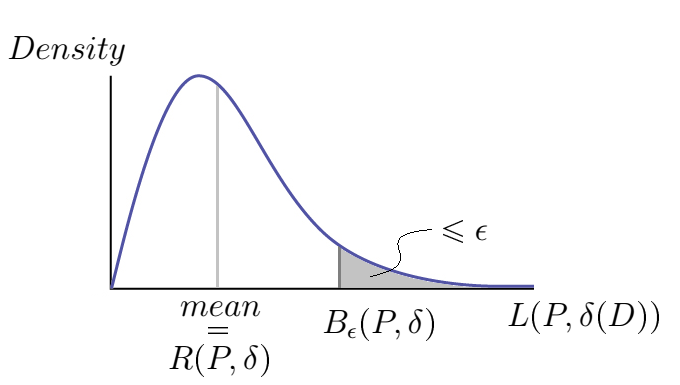
\includegraphics[scale=0.5]{graph_3.png}}

\subsubsection{Comparing Decision Rules}
We would like to be able to compare rules together to figure out which one to choose. If we could find a rule that dominates all the other rules, we would choose this rule. But often, we can't find such a rule. \emph{This is why there is no universally best procedure.} The frequentist approach is to analyze different properties of decision rules, and the user can then choose which one they prefer according to which properties is better to them.

We now present two standard ways in statistics to reduce a risk profile curve to a scalar, and so we can then compare rules together and get a notion of "optimality":

\begin{enumerate}[A)]
\item \emph{The Minimax Criteria}:\\
Following this criteria, the optimal rule $\delta^*$ is given by:
$$\delta^*_{minimax}=\text{arg}\,\min\limits_{\delta}\,\max\limits_{P \in \mathcal{P}}\ R(P,\delta)$$

In words, the minimax optimal rule is the rule who minimizes the \textit{risk} we would obtain in the worst possible scenario.

\item \emph{Weighting}:\\
This criteria requires that we define a \emph{weighting} over $\Theta$ (can be interpreted as a prior). Formally:
$$\delta^*_{weight}= \text{arg}\,\min\limits_{\delta}\,\int_{\Theta}^{}R(P_\theta,\delta)\pi(\theta)d\theta$$

Intuitively, when considering a certain rule, we are averaging the risk over all the possible $\theta$ by putting more weight on the $\theta$ we believe are more important for the phenomenon that we are studying. After that, we can compare them with each other and pick the rule corresponding to the lowest average.

\item \emph{Bayesian Statistical Decision Theory}:\\
The last two criteria were not making any use of the fact that we observed data (that we observed a realization of $D$). The \textit{bayesian optimality criteria} makes use of this information. Before defining this criteria, let's define what we call the \textit{bayesian posterior risk}:
$$R_B(\delta|D) \triangleq \int_{\Theta}^{}L(P_{\theta},\delta)p(\theta|D)d\theta,$$
where $p(\theta|D)$ is the posterior for a given prior $\pi(\theta)$.

The optimal rule following the bayesian criteria is:
$$\delta_{bayes}^{*}(D)= \text{arg}\,\min\limits_{\delta}\,R_B(\delta|D)$$
As you recall, in the Bayesian philosophy, we treat all uncertain quantities with probabilities. The posterior on $\theta$ summarizes all the information we need about the uncertain quantity $\theta$. As a Bayesian, the statistical loss $L(\theta,a)$ then tells us how we can \emph{act optimally}: we simply need to find the action that minimizes the Bayesian posterior risk (as $\theta$ is integrated out, there is no more uncertainty about $\theta$!). $\delta_{bayes}^{*}$ is thus the \textit{only} procedure to use as a Bayesian! Life is quite easy for a Bayesian (no need to worry about other properties like minimax, frequentist risk, etc.). The Bayesian does not care about what could happen for other $D$'s, it only cares that you are given a specific observation $D$, and want to know how to act \textit{given} $D$.

But a frequentist can still decide to analyze a Bayesian procedure from the frequentist risk perspective. In particular, one can show that most Bayesian procedures are admissible (unlike the MLE!). Also, one can show that the Bayesian procedure is the \textit{optimal} procedure when using the weighted risk summary with weight function $\pi(\theta)$ which matches the prior $p(\theta)$. This can be seen as a simple application of Fubini's theorem, and from the diamond graph below: \\
\centerline{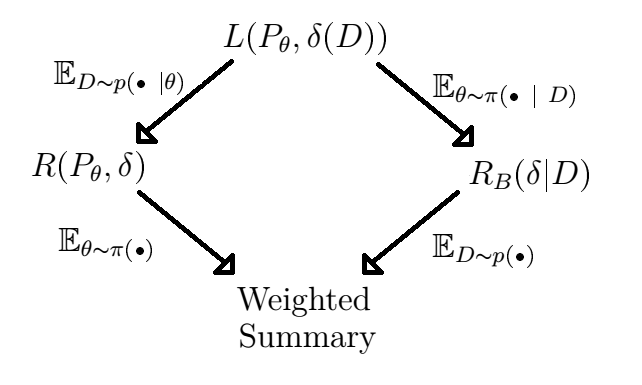
\includegraphics[scale=0.5]{graph_2.png}}
where $p(\bullet\ | \theta)$ stands for $D$'s pdf conditional to  $\theta$, where $p(\bullet) = \int_{\Theta}^{}p(\bullet\ | \theta)\pi(\theta )d\theta$ and where $\pi(\cdot | D)$ denotes the posterior on $\theta$.
The bayesian procedure has the property that it minimizes the weighted summary.

\end{enumerate}

\noindent\textit{\textbf{Exercise :}}\\
Given $\mathcal{A} = \Theta$ and $L(\theta,a)=\norm{\theta-a}^2$, show that $\delta_{bayes}^{*}(D) = \E[\theta|D]$ (the posterior mean).
\subsubsection{Examples of Estimators}
\begin{enumerate}
\item Maximum likelihood estimator (MLE)
$$\delta_{MLE}(D)= \hat{\theta}_{MLE} = \text{arg}\,\max\limits_{\theta} \mathcal{L}_D(\theta)$$
where $\mathcal{L}_D(\theta)$ is the likelihood function given the observation $D$.
\item Maximum a posteriori (MAP)
$$\delta_{MAP}(D)= \hat{\theta}_{MAP} = \text{arg}\,\max\limits_{\theta} \pi(\theta|D)$$
where $\pi(\theta|D)$ is the \textit{posterior distribution} over all the possible $\theta$. 
\item Method of Moments\\
Suppose we have that $D = (X_1,...,X_n)$ with $X_i \thicksim^{iid} P_\theta$ being scalar random variables where $\theta$ is a vector (i.e. $\theta = (\theta_1,...,\theta_k)$). 
The idea is to find an bijective function $h$ that maps any $\theta$ to  the "vector of moments" (i.e. $M_k(X_1)=(\E[X_1],\E[X_1^2],...,\E[X_1^k])$). Basically,
$$h(\theta)=M_k(X_1)$$
Since $h$ is bijective, we can invert it,
$$h^{-1}(M_k(X_1)) = \theta$$
The intuition is that to approximate $\theta$, we could evaluate the function $h^{-1}$ using as input the \textit{empirical moments} vector (i.e. $\hat{M}_k(X_1)= (\hat{\E}[X_1],\hat{\E}[X_1^2],...,\hat{\E}[X_1^k])$ where $\hat{\E}[X_1^j] \triangleq \frac{1}{n}\sum_{i}x_i^j$ for a given $j$). This would be our \textit{method of moments estimator}:
$$h^{-1}(\hat{M}_k(X_1)) = \hat{\theta}_{MM}$$

\textbf{\textit{Example:}}\\
Suppose that $X_i \thicksim^{iid} \mathcal{N}(\mu,\sigma^2)$. We have that,
$$\E[X_1]=\mu$$
$$\E[X_1^2]=\sigma^2+\mu^2$$

This defines our function $h$. Now, we invert the relation:

$$\mu = \E[X_1]$$
$$\sigma^2 = \E[X_1^2] + \E^2[X_1]$$

Then, we finally replace the moments by the empirical moments to get our estimator:

$$\hat{\mu}_{MM} = \hat{\E}[X_1]$$
$$\hat{\sigma}^2_{MM} = \hat{\E}[X_1^2] + \hat{\E}^2[X_1]$$

Here, this MM estimator is the same as the ML estimator. This illustrates a property of the exponential family (we will see this later in this class).

Note: The method of moment is quite useful for latent variable models (e.g. mixture of Gaussian), see ``spectral methods'' or ``tensor decomposition'' methods in the recent literature\footnote{See: ``Tensor Decompositions for Learning Latent Variable Models'', by Anandkumar et al., \href{http://jmlr.org/papers/v15/anandkumar14b.html}{JMLR 2014} e.g.}.

\item ERM for prediction function estimation\\
In this context, $\mathcal{A}= \mathcal{F} \subset \mathcal{Y}^\mathcal{X}$ and the decision rule is a function $\delta: \mathcal{D} \mapsto \mathcal{Y}^\mathcal{X}$. $\mathcal{F}$ is called the \textit{hypothesis space}. We are looking for a function $f^*\in \mathcal{Y}^\mathcal{X}$ that minimizes the \textit{generalization error}. Formally,

$$f^*=\text{arg}\,\min\limits_{f \in \mathcal{Y}^\mathcal{X}} \E_{D \thicksim P}[l(y,f(x))]$$

Since we don't know what is $P$, we can't compute $\E_{D \thicksim P}[l(y,f(x))]$. As a replacement, we consider $\hat{f}_{ERM}$ an estimator of $f^*$:

$$\hat{f}_{ERM} = \text{arg}\,\min\limits_{f \in \mathcal{F}} \hat{\E}[l(y,f(x))]$$

where $\hat{\E}[l(y,f(x))]= \frac{1}{n}\sum_{i = 1}^n l(y_i,f(x_i)) $. ERM stands for \textit{empirical risk minimizer} (here, the Vapnik risk).

\end{enumerate}

\subsection{Convergence of random variables}
\subsubsection{Convergence in distribution}
In general, we say that a sequence of random variable $\{X_n\}_{n=1}^\infty$ \textit{converges in distribution} towards a random variable $X$ if 
$$\lim_{n \to \infty}F_n(x)=F(x)\ \forall x$$
where $F_n$ and $F$ correspond the cumulative functions of $X_n \forall n$ and of $X$ respectively.
In such a case, we note $X_n \xrightarrow[]{d} X$

\subsubsection{Convergence in $L_k$}
In general, we say that a sequence of random variable $\{X_n\}_{n=1}^\infty$ \textit{converges in the $L_k\ norm$} towards a random variable $X$ if 
$$\lim_{n \to \infty}\E[\ \norm{X_n-X}^k_k]=0$$
In such a case, we note $X_n \xrightarrow[]{L_k} X$

\subsubsection{Convergence in Probability}

In general, we say that a sequence of random variable $\{X_n\}_{n=1}^\infty$ \textit{converges in probability} towards a random variable $X$ if 
$$\forall \epsilon>0,\ \lim_{n \to \infty}P\{\norm{X_n-X}\geq \epsilon\}=0$$
In such a case, we note $X_n \xrightarrow[]{p} X$.\\

Note: It turns out that \textit{$L_2$ convergence} implies \textit{convergence in probability}. (The reverse implication isn't true)

\subsection{Properties of estimator}
Suppose that $D_n = (X_1, ..., X_n)$ and that $X_i \thicksim^{iid} P_\theta$. We will note $\hat{\theta}_n=\delta_n(D_n)$ an estimator of $\theta$. The subscript stands to emphasize the fact that the estimator's value depends on the number of observation $n$.

\subsubsection{Bias of an estimator}
$$Bias(\hat{\theta}_n) = \E[\hat{\theta}_n - \theta]$$

\subsubsection{Standard Statistical Consistency}
We say that an estimator $\hat{\theta}_n$ is consistent for a parameter $\theta$ if $\hat{\theta}_n$ converges in probability toward $\theta$ (i.e. $\hat{\theta}_n \xrightarrow[]{p} \theta$).

\subsubsection{$L_2$ Consistency}
We say that an estimator $\hat{\theta}_n$ is $L_2$ consistent for a parameter $\theta$ if $\hat{\theta}_n$ converges in $L_2$ norm toward $\theta$ (i.e. $\hat{\theta}_n \xrightarrow[]{L_2} \theta$).

\subsubsection{Bias-variance decomposition}
Consider $L(\theta,\hat{\theta}_n)=\norm{\theta - \hat{\theta}_n}^2_2$. We will express the frequentist \textit{risk} as a function of the bias and variance of $ \hat{\theta}_n$.\\

\begin{align}
R(P_\theta,\delta_n) &= \E_{D \thicksim P_\theta}[\ \norm{\theta - \hat{\theta}_n}^2]\\
&=\E[\ \norm{\theta -\E[\hat{\theta}_n] + \E[\hat{\theta}_n] - \hat{\theta}_n}^2]\\
&=\E[\ \norm{\theta -\E[\hat{\theta}_n]}^2] + \E[\ \norm{\E[\hat{\theta}_n] - \hat{\theta}_n}^2] + 2\E[\ \langle\theta-\E[\hat{\theta}_n],\E[\hat{\theta}_n] - \hat{\theta}_n\rangle]\\
&=\E[\ \norm{\theta -\E[\hat{\theta}_n]}^2] + \E[\ \norm{\E[\hat{\theta}_n] - \hat{\theta}_n}^2] + 2\langle\theta-\E[\hat{\theta}_n],\E[\hat{\theta}_n] - \E[\hat{\theta}_n]\rangle\\
&=\norm{\theta -\E[\hat{\theta}_n]}^2 + \E[\ \norm{\E[\hat{\theta}_n] - \hat{\theta}_n}^2]\\
&=\norm{bias(\hat{\theta}_n)}^2 + Var[\hat{\theta}_n]
\end{align}
Remark: Other loss functions would have potentially led to a different function of the bias and the variance, thus expressing a different priority between the bias and the variance.

\centerline{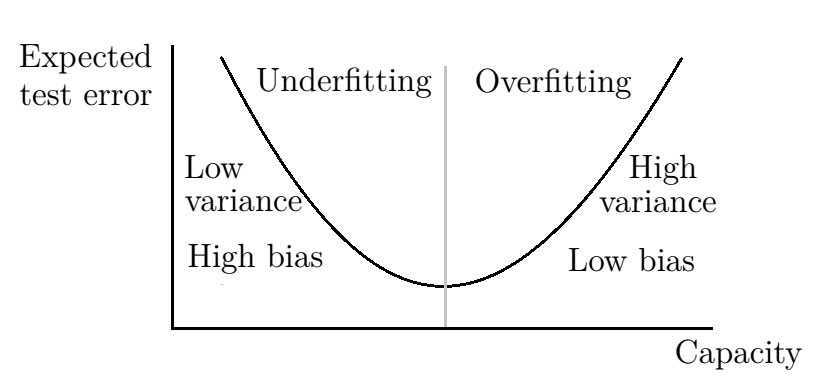
\includegraphics[scale=0.5]{graph_4.png}}

\subsubsection{The James-Stein estimator}
The \href{https://en.wikipedia.org/wiki/James-Stein\_estimator}{\textit{James-Stein estimator}} for estimating the mean of a $X_i \thicksim^{iid}\mathcal{N}_d(\mu,\sigma^2I)$ \textit{dominates} the MLE estimator for the \textit{squared loss} when $d\geq 3$ (and thus showing that the MLE is inadmissible in this case). It turns out that the James-Stein estimator is biased, but that its variance is sufficiently smaller than the MLE's variance to offset the bias.

\subsubsection{Properties of the MLE}
Assuming sufficient regularity conditions on $\Theta$ and $p(x; \theta)$, we have:
\begin{enumerate}
\item Consistent: $\hat{\theta}_{MLE} \xrightarrow[]{p} \theta$
\item CLT: $\sqrt{n}(\hat{\theta}_{MLE}-\theta) \xrightarrow[]{d} \mathcal{N}(0,I(\theta)^{-1}) $ where $I$ is the 
\href{https://en.wikipedia.org/wiki/Fisher\_information\#Matrix\_form}{\textit{Fisher information matrix}}.
\item Asymptotic optimality:\\
Among all unbiased estimator of a scalar parameter $\theta$, $\hat{\theta}_{MLE}$ is the one with the lowest variance asymptotically. \\This results follows from the \href{https://en.wikipedia.org/wiki/Cram\%C3\%A9r-Rao\_bound}{\textit{Cramér-Rao bound}} result, which can be stated like this: Let $\hat{\theta}$ be an unbiased estimator of a scalar parameter $\theta$. Then we have that,
$$Var[\hat{\theta}]\geq \frac{1}{I(\theta)}$$
Note that this result can also be stated in the multivariate case.
\item Invariance to reparametrization:\\
Suppose we have a bijection $f:\Theta \mapsto \Theta$, then,
$$\widehat{f(\theta)}_{MLE} = f(\hat{\theta}_{MLE})$$

This result can be generalized to the case where $f$ isn't a bijection.\\
Suppose $g: \Theta \mapsto \Lambda$ (bijective or not). We define the \textit{profile likelihood}:
$$L(\eta) \triangleq \max\limits_{\theta | \eta = g(\theta)}p(data;\theta)$$
Let also define the generalized MLE in this case as:
$$\hat{\eta}_{MLE} \triangleq \text{arg}\,\max\limits_{\eta \in g(\Theta)}L(\eta)$$
Then we have that
$$\hat{\eta}_{MLE} = g(\hat{\theta}_{MLE})$$
this is called a \emph{plug-in estimator} because you are simply ``plugging in'' the value $\hat{\theta}_{MLE}$ in the function $g$ to get its MLE.

\textbf{\textit{Examples}}
\begin{enumerate}
\item $\widehat{\sigma^2}_{MLE} = (\hat{\sigma}_{MLE})^2$
\item $(\widehat{\sin\sigma^2})_{MLE} = \sin(\hat{\sigma^2}_{MLE})$
\end{enumerate}

\end{enumerate}


\end{document}
